\subsection{Анализ архитектурных подходов и технологий для построения серверных приложений}
\label{sec:analysis:research:mobArch}

Современные серверные приложения предполагают использование архитектуры и инструментов, позволяющие

\begin{itemize}
\item получить высокую тестируемость приложения;
\item быстро и стабильно разворачивать всю инфраструктуру приложения;
\item с минимальными затратами масштабировать приложение;
\item получить надёжность и отказоустойчивость.
\end{itemize}

Существуют два основных подхода при разработке серверных приложений, которые будут рассмотрены в следующих параграфах: монолит и микросервисы.

\paragraph {} Монолитная архитектура
Монолитная архитектура предполагает развёртывание приложения одним файлом(например, WAR фаил) или архивом файлов(например, приложение на Rails), все модули приложения разрабатываются, развёртываются и тестируются одновременно. Обычно при реализации данного подхода, всё приложение использует одну базу данных. На рисунке \ref{sec:analysis:research:arch:back:monolith} представлен пример организации монолитного приложения. \cite{microservices:ma}

\begin{figure}[h]
  \centering
    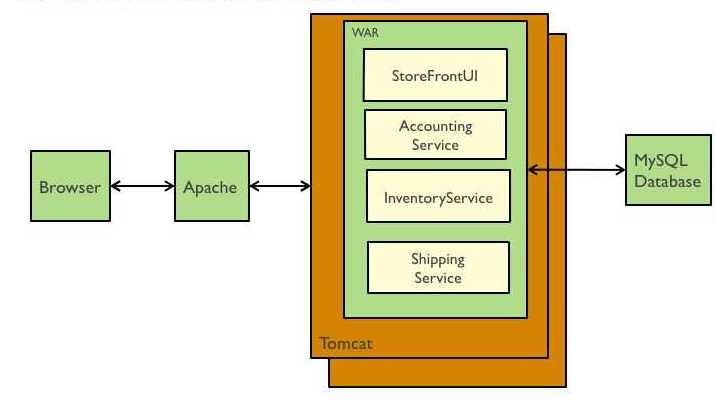
\includegraphics[width=1\textwidth]{inc/img/backend-monolith.jpg}
  \caption{Пример организации монолитного серверного приложения}
  \label{sec:analysis:research:arch:back:monolith}
\end{figure}

К плюсам подхода можно отнести:

\begin{enumerate}
	\item \emph{Простота в разработке} --- целью современных \gls{ide} является поддержка монолитных приложений.
	\item \emph{Простота в развёртывании} --- для старта работы всего приложения нужно лишь запустить один процесс с подготовленным окружением.
	\item \emph{Простота в масштабируемости} --- приложение масштабируется путём запуска дополнительных процессов приложения, организованных при помощи балансировщика нагрузки.
\end{enumerate}

Данный подход удобен до определённого размера приложения, однако, чем больше и сложнее становится приложение, тем существенней становятся следующие проблемы:

\begin{enumerate}
	\item \emph{Сложность поддержки} --- с увеличением кодовой базы, увеличивается сложность ввода нового специалиста в проект. Результатом является общее замедление разработки и отсутствие возможности быстро ускорить разработку при помощи привлечения дополнительных специалистов.
	\item \emph{Перегруженная \gls{ide}} --- хотя современные \gls{ide} и ориантируются на монолитные приложения, большая кодовая база способна сильно замедлить работу \gls{ide}.
	\item Долгий запуск контейнера приложения.
	\item \emph{Сложности при масштабировании} --- на определённом этапе, в приложении появляются слабые точки производительности. Часто таких точек несколько и они трубуют разные виды ресурсов(база, процессор, память), однако единственный способ масштабировать приложение --- запускать новый процесс со всем приложением внутри, что не позволяет точечно устранять проблемы.
	\item \emph{Привязанность к технологическому стеку} --- монолитное приложение крайне сложно постепенно переводить на новый технологический стек, а единовременное полное портирование приложения -- опасный процесс, производящий огромное количество ошибок.
\end{enumerate}
\subsubsection {}
\label{sec:analysis:research:backArch:microservices}

Микросервисная архитектура предлагает рассматривать приложение как набор слабо связанных сервисов, взаимодействующих друг с другом. Каждый сервис реализует фокусированный набор связанных функций. Например, приложение может содержать сервисы для авторизации, отправки сообщений, пуш-уведомлений.

Сервисы могут общаться при помощи как синхронных, так и асинхронных протоколов, часто выбор ложится на HTTP/REST. Такой подход позволяет разрабатывать и разворачивать сервисы независимо друг от друга, каждый сервис имеет собственную базу данных, консистентность данных между сервисами поддерживается при помощи паттерна Saga. \cite{microservices:ms}

На рисунке \ref{sec:analysis:research:arch:back:micro} представлен пример организации микросервисного приложения.

\begin{figure}[h]
  \centering
    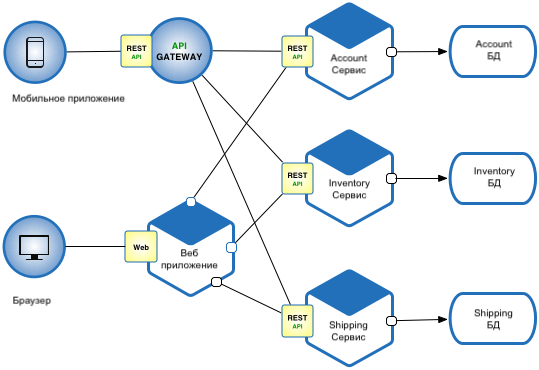
\includegraphics[width=1\textwidth]{inc/img/backend-micro.png}
  \caption{Пример организации монолитного серверного приложения}
  \label{sec:analysis:research:arch:back:micro}
\end{figure}

Очевидными плюсами микросервисного подхода являются:

\begin{enumerate}
	\item \emph{Тестируемость} --- небольшие сервисы проще тестировать в изолированной среде.
	\item \emph{Скорость развёртывания} --- небольшой сервис разворачивается намного быстрее полноценного приложения.
	\item \emph{Модульность} --- микросервисная архитектура значительно упрощает разделение сотрудников на команды.
	\item \emph{Меньший порог входа} --- разработчику нужно разбираться только с одним небольшим сервисом.
	\item \emph{Скорость разработки} --- отсутствие неявных зависимостей, скорость развёртывания и скорость работы \gls{ide} положительно сказываются на продуктивности разработчиков.
	\item \emph{Повышенная отказоустойчивость} --- выход из строя одного сервиса не выведет из строя всё приложение.
	\item \emph{Гибкость масштабирования} --- разработчики получают возможность масштабировать отдельно сервисы.
	\item \emph{Гибкость в выборе технологического стека} --- каждый сервис может быть разработан, используя собственный технологический стек, переход на новую технологию можно выполнять поэтапно.
\end{enumerate}

Однако, микросервисная архитектура значительно повышает общую сложность системы, вводя дополнительную работу для программистов:

\begin{enumerate}
	\item \emph{Отсутствие поддержки со стороны \gls{ide}} --- если перед разработчиком стоит задача, которая предполагает изменение нескольких сервисов --- \gls{ide} будет неспособна работать над несколькими проектами одновременно.
	\item Появляется необходимость разработки и поддержки протокола общения между сервисами.
	\item Перед разработчиками появляются задачи координации сервисов, аггрегации запросов.
	\item \emph{Усложнённый процесс запуска всего приложения} --- для запуска всего приложения требуется развернуть каждый сервис отдельно.
	\item \emph{Повышенное потребление ресурсов} --- каждый сервис является отдельным процессом, поэтому ресурсы, которые тратятся на поддержку работоспособности процесса увеличиваются на количество сервисов.
\end{enumerate}

% Так как каждый сервис имеет собственную базу данных, а часто бизнес-логика требует работы сразу нескольких сервисов, стоит рассмотреть механизмы для аггрегации запросов между сервисами и поддержки консистентности состояния.

% -- Api Composition
% -- Saga pattern